\documentclass{beamer}
\usepackage[utf8]{inputenc}
\usepackage{graphicx, epsfig}
\usepackage{amsmath,mathrsfs,amsfonts,amssymb}
%\usepackage{subfig}
\usepackage{floatflt}
\usepackage{epic,ecltree}
\usepackage{mathtext}
\usepackage{fancybox}
\usepackage{fancyhdr}
\usepackage{multirow}
\usepackage{enumerate}
\usepackage{epstopdf}
\usepackage{multicol}
\usepackage{algorithm}
\usepackage[noend]{algorithmic}
\def\algorithmicrequire{\textbf{Input:}}
\def\algorithmicensure{\textbf{Output:}}
\usetheme{default}%{Singapore}%{Warsaw}%{Warsaw}%{Darmstadt}
\usecolortheme{default}
\setbeamertemplate{footline}[page number]{}
\setbeamerfont{title}{size=\Huge}

\newcommand{\bc}{\mathbf{c}} 
\newcommand{\bt}{\mathbf{t}} 
\newcommand{\bu}{\mathbf{u}} 
\newcommand{\bv}{\mathbf{v}} 
\newcommand{\bw}{\mathbf{w}} 
\newcommand{\bx}{\mathbf{x}} 
\newcommand{\bz}{\mathbf{z}} 
\newcommand{\by}{\mathbf{y}} 

\newcommand{\bI}{\mathbf{I}} 
\newcommand{\bT}{\mathbf{T}} 
\newcommand{\bX}{\mathbf{X}} 
\newcommand{\bZ}{\mathbf{Z}} 

\newcommand{\bepsilon}{\boldsymbol{\epsilon}}
\newcommand{\bmu}{\boldsymbol{\mu}}
\newcommand{\blambda}{\boldsymbol{\lambda}}
\newcommand{\bsigma}{\boldsymbol{\sigma}}
\newcommand{\bSigma}{\boldsymbol{\Sigma}}

\newcommand{\bbE}{\mathbb{E}} 
\newcommand{\bbP}{\mathbb{P}} 
\newcommand{\bbR}{\mathbb{R}} 

\newcommand{\cL}{\mathcal{L}} 
\newcommand{\cN}{\mathcal{N}} 
\newcommand{\cS}{\mathcal{S}} 
\newcommand{\cX}{\mathcal{X}} 

\newcommand{\btheta}{\boldsymbol{\theta}} 
\newcommand{\bphi}{\boldsymbol{\phi}} 

\DeclareMathOperator*{\argmin}{arg\,min}
\DeclareMathOperator*{\argmax}{arg\,max}

%\definecolor{beamer@blendedblue}{RGB}{15,120,80}
%----------------------------------------------------------------------------------------------------------
\title[\hbox to 56mm{Deep Generative Models  \hfill\insertframenumber\,/\,\inserttotalframenumber}]
{Deep Generative Models \\ Lecture 11}
\author[Roman Isachenko]{\\Roman Isachenko}
\institute[MIPT]{Moscow Institute of Physics and Technology \\
}
\date{2020}
%--------------------------------------------------------------------------------
\begin{document}
%--------------------------------------------------------------------------------
\begin{frame}
%\thispagestyle{empty}
\titlepage
\end{frame}
%=======
\begin{frame}{Disentangled representations}
\begin{block}{Goal}
    Learning an interpretable factorised representation of the independent data generative factors of the world without supervision. 
\end{block}
\begin{block}{Informal definition}
A disentangled representation can be defined as one where single latent units are sensitive to changes in single generative factors, while being relatively invariant to changes in other factors. 
\end{block}
\begin{block}{Example}
Model trained on a dataset of 3D objects might learn independent latent units sensitive to single independent data generative factors, such as object identity, position, scale, lighting or colour. 
\end{block}
\vfill
\hrule\medskip
{\scriptsize \href{https://openreview.net/references/pdf?id=Sy2fzU9gl}{https://openreview.net/references/pdf?id=Sy2fzU9gl}}
\end{frame}
%=======
\begin{frame}{$\beta$-VAE, 2017}
\begin{block}{Generative process}
\begin{itemize}
    \item $p(\bx | \bv, \bw) = \text{Sim}(\bv, \bw)$~-- true world simulator;
    \item $\bv$~-- conditionally independent factors: $p(\bv | \bx) = \prod_{k=1}^K p(v_k | \bx)$;
    \item $\bw$~-- conditionally dependent factors. 
\end{itemize}
\end{block}
\begin{block}{Goal}
Develop an unsupervised deep generative model
\[
    p(\bx | \bz) \approx p(\bx | \bv, \bw).
\]
\vspace{-0.5cm}
\begin{itemize}
    \item Ensure that the inferred latent factors $q(\bz|\bx)$ capture the factors $\bv$ in a disentangled manner. 
    \item The conditionally dependent factors $\bw$ can remain entangled in a separate subset of $\bz$ that is not used for representing $\bv$. 
\end{itemize}
\end{block}
\vfill
\hrule\medskip
{\scriptsize \href{https://openreview.net/references/pdf?id=Sy2fzU9gl}{https://openreview.net/references/pdf?id=Sy2fzU9gl}}
\end{frame}
%=======
\begin{frame}{InfoGAN}
	\begin{block}{GAN objective}
		\vspace{-0.3cm}
		\[
		\min_{G} \max_D V(G, D)
		\]
		\[
		V(G, D)  =  \bbE_{\pi(\bx)} \log D(\bx) + \bbE_{p(\bz)} \log (1 - D(G(\bz)))
		\]
	\end{block}
	Latent vector $\bz$ is not imposed to be disentangled.
	
	InfoGAN decomposes input vector:
	\begin{itemize}
		\item $\bz$ -- incompressible noise;
		\item $\bc$ -- structured latent code.
	\end{itemize}
	\begin{block}{Information-theoretic regularization}
		\vspace{-0.3cm}
		\[
			\max I (\bc, G(\bz, \bc))
		\]
	\end{block}
	Information in the latent code $\bc$ should not be lost in the generation process.
	\vfill
	\hrule\medskip
	{\scriptsize \href{https://arxiv.org/abs/1606.03657}{https://arxiv.org/abs/1606.03657}}
\end{frame}
%=======
\begin{frame}{InfoGAN}
	\begin{block}{Objective}
		\vspace{-0.3cm}
		\[
		\min_{G} \max_D V(G, D) - \lambda I (\bc, G(\bz, \bc))
		\]
	\end{block}
	\begin{block}{Variational Information Maximization}
		\begin{multline*}
		I (\bc, G(\bz, \bc)) = H(\bc) - H(\bc | G(\bz, \bc)) = \\
		= H(\bc) + \bbE_{\bx \sim G(\bz, \bc)} \left[ \bbE_{\bc \sim p(\bc | \bx)} \log p(\bc' | \bx) \right] = \\ 
		= H(\bc) + \bbE_{\bx \sim G(\bz, \bc)} KL(p(\bc'| \bx) || q(\bz' | \bx)) + 
		\\ + \bbE_{\bx \sim G(\bz, \bc)}  \bbE_{\bc' \sim p(\bc | \bx)} \log q(\bc' | \bx)  \geq\\
		 \geq H(\bc) + \bbE_{\bx \sim G(\bz, \bc)} \bbE_{\bc' \sim p(\bc | \bx)} \log q(\bc' | \bx) = \\
		 H(\bc) + \bbE_{\bc \sim p(\bc)} \bbE_{\bx \sim G(\bz, \bc)} \log q(\bc' | \bx)
		\end{multline*}
	\end{block}
	\vfill
	\hrule\medskip
	{\scriptsize \href{https://arxiv.org/abs/1606.03657}{https://arxiv.org/abs/1606.03657}}
\end{frame}
%=======
\begin{frame}{InfoGAN}
	\begin{block}{Latent codes on MNIST}
		\begin{figure}
			\centering
			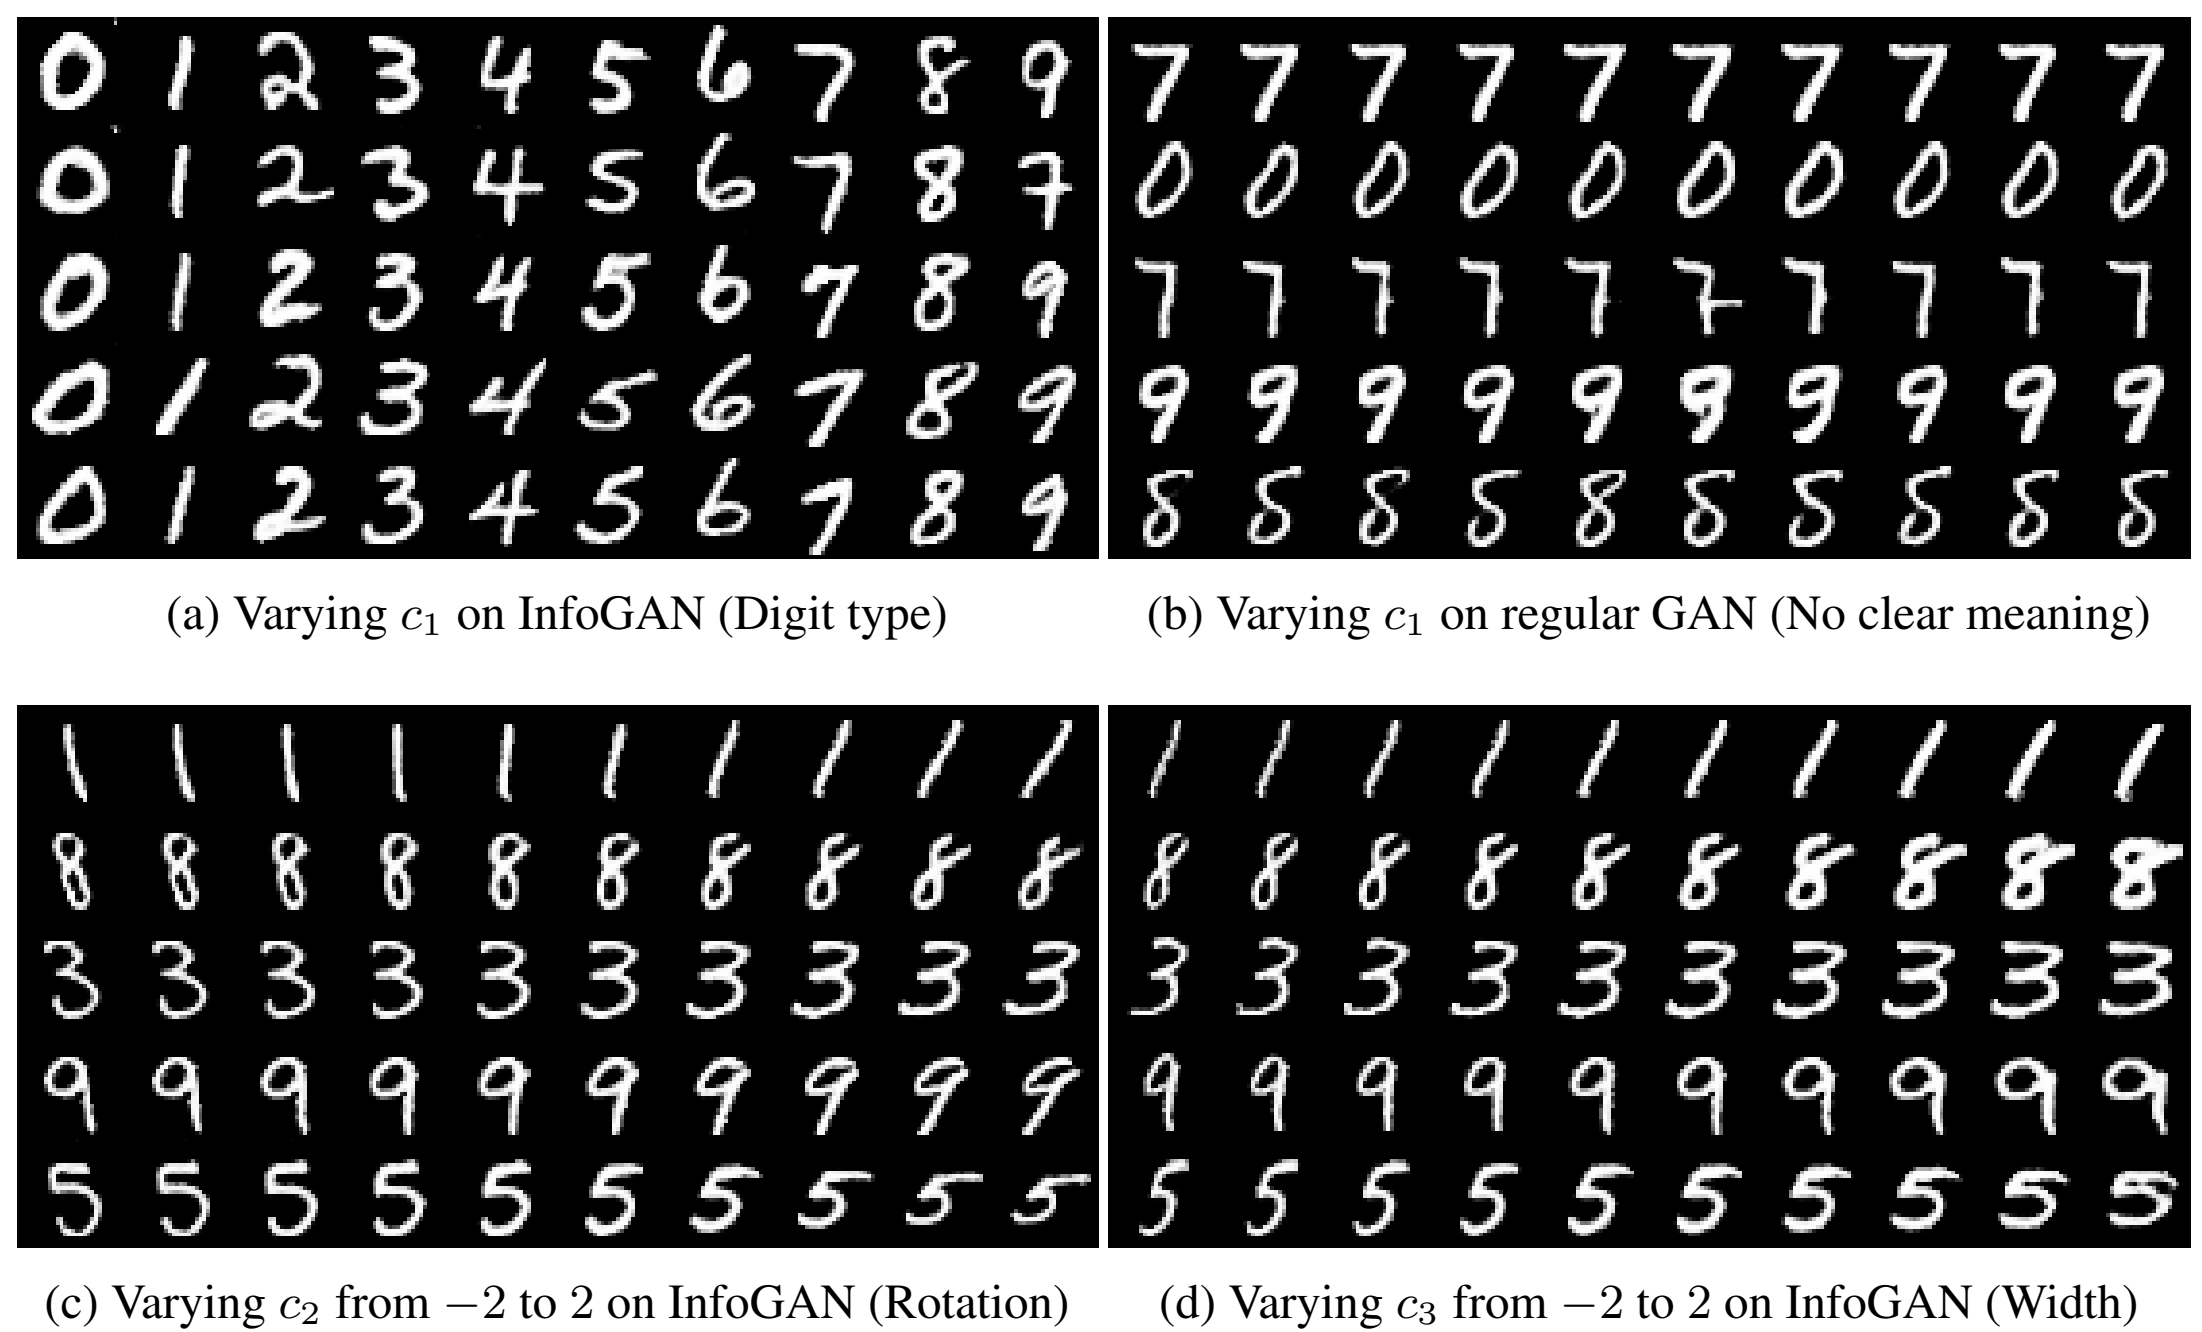
\includegraphics[width=\linewidth]{figs/infogan_mnist.png}
		\end{figure}
	\end{block}
	\vfill
	\hrule\medskip
	{\scriptsize \href{https://arxiv.org/abs/1606.03657}{https://arxiv.org/abs/1606.03657}}
\end{frame}
%=======
\begin{frame}{InfoGAN}
	\begin{block}{Latent codes on 3D Faces}
		\begin{figure}
			\centering
			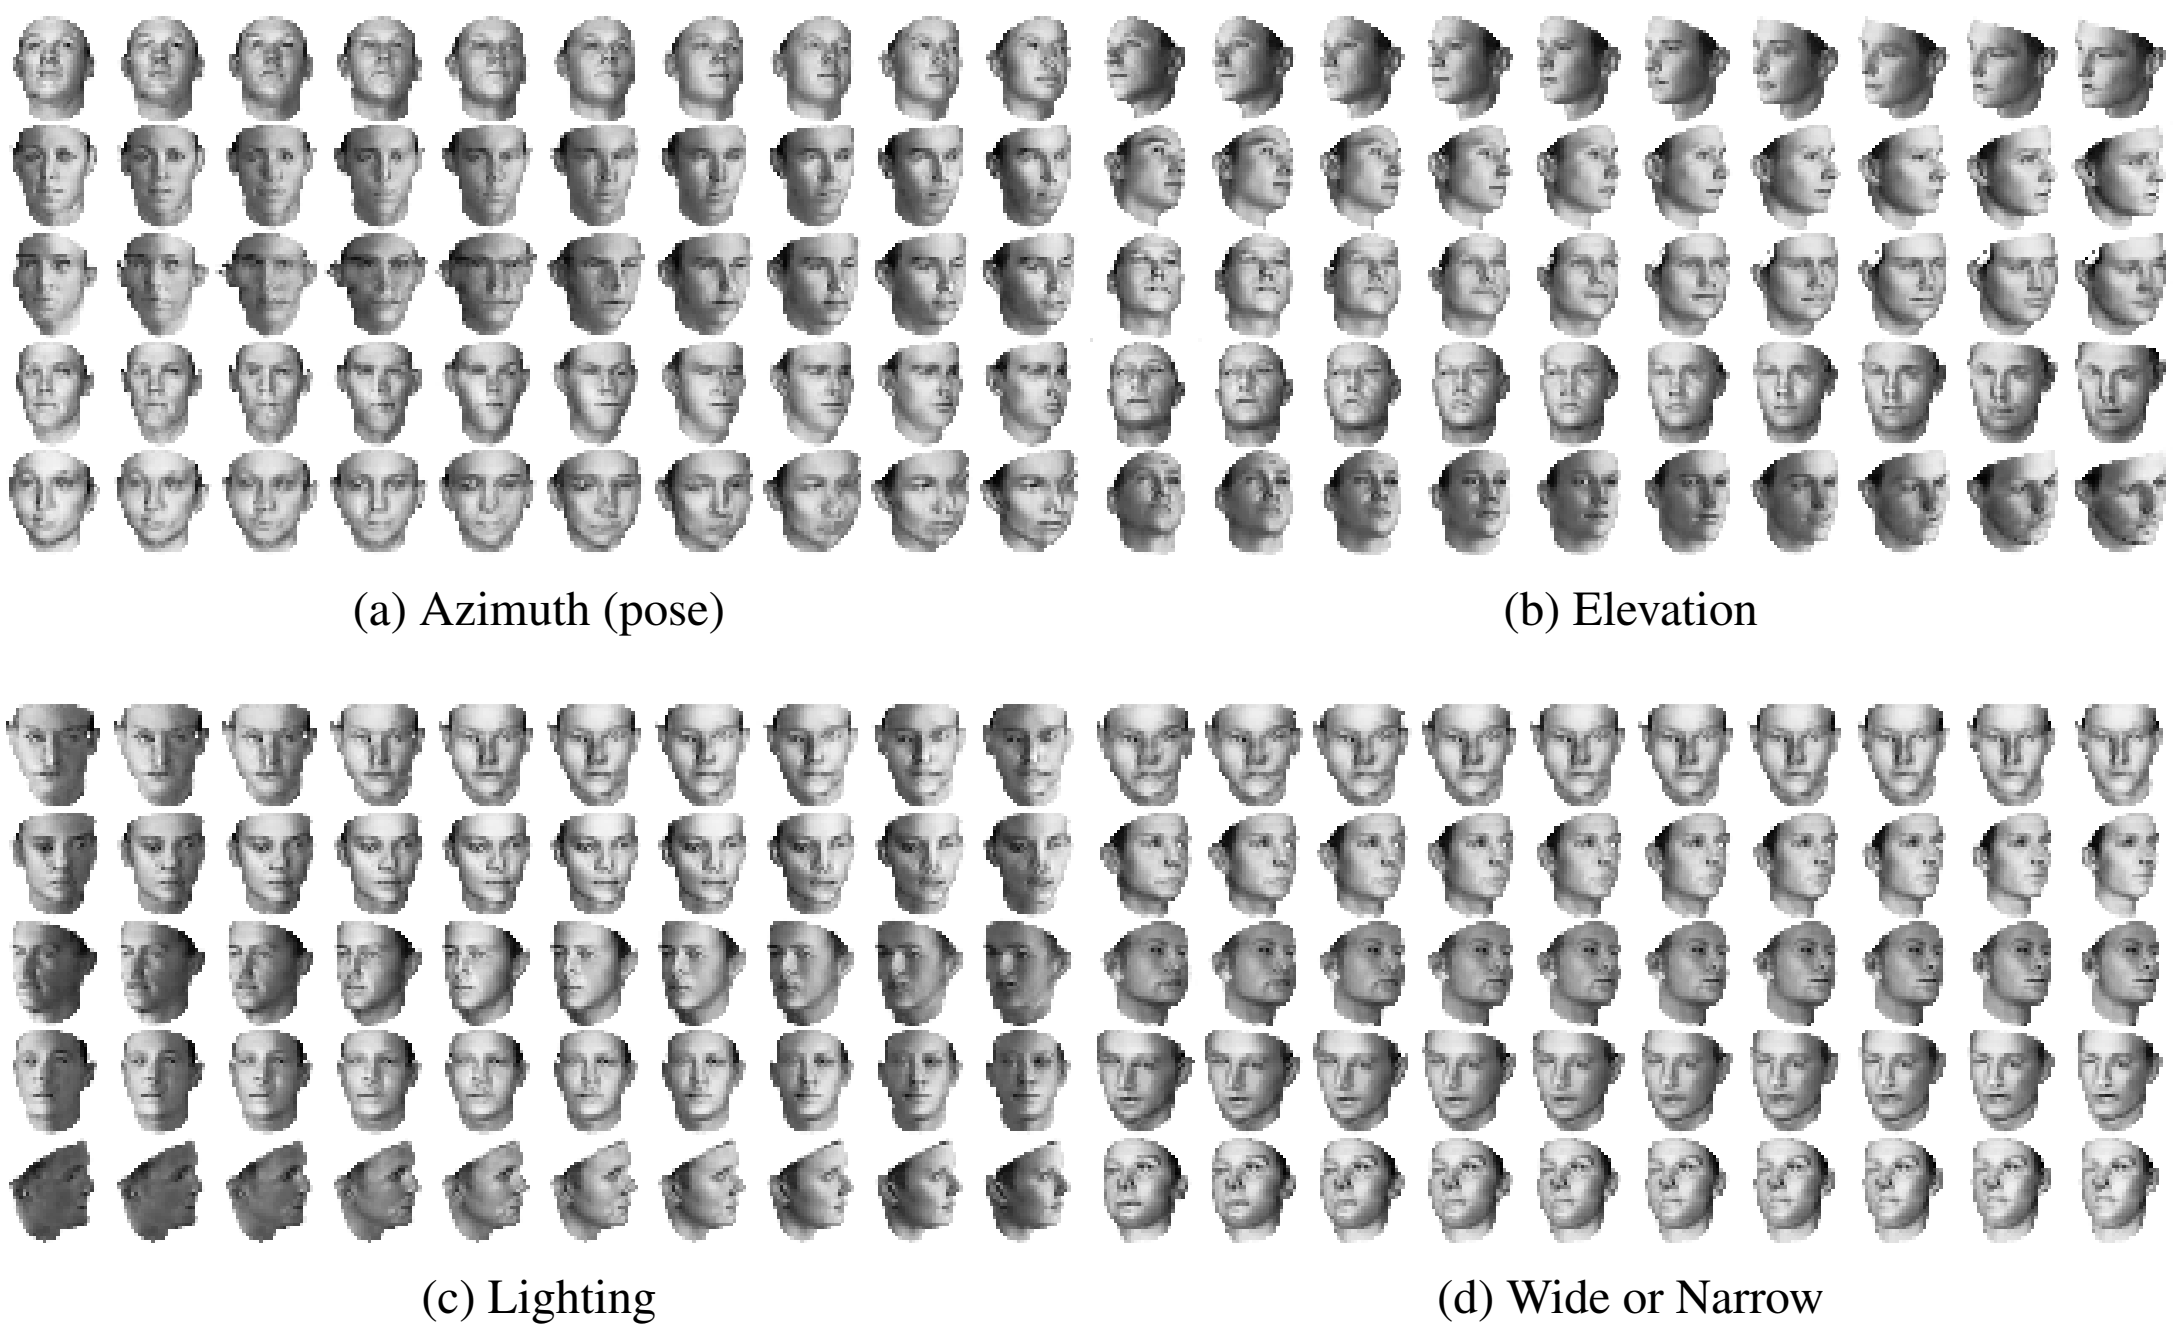
\includegraphics[width=\linewidth]{figs/infogan_faces.png}
		\end{figure}
	\end{block}
\vfill
\hrule\medskip
{\scriptsize \href{https://arxiv.org/abs/1606.03657}{https://arxiv.org/abs/1606.03657}}
\end{frame}
%=======
\begin{frame}{$\beta$-VAE, 2017}
\begin{block}{Constrained optimization}
\vspace{-0.5cm}
\[
    \max_{q, \btheta} \mathbb{E}_{q(\bz | \bx)} \log p(\bx | \bz, \btheta), \quad \text{subject to } KL (q(\bz | \bx) || p(\bz)) < \epsilon.
\]
\vspace{-0.5cm}
\end{block}
\begin{block}{Objective}
\vspace{-0.5cm}
\[
    \mathcal{L}(q, \btheta, \beta) = \mathbb{E}_{q(\bz | \bx)} \log p(\bx | \bz, \btheta) - \beta \cdot KL (q(\bz | \bx) || p(\bz)).
\]
\end{block}
What do we get at $\beta = 1$? \\
\begin{block}{Hypothesis}
To learn disentangled representations of the conditionally independent factors $\bv$, it is important to set stronger constraint on the latent bottleneck: $\beta > 1$.
\end{block}
\textbf{Note:} It could lead to poorer reconstructions due to the loss of high frequency details when passing through a constrained latent bottleneck. \\ 
\vspace{0.1cm}
\vfill
\hrule\medskip
{\scriptsize \href{https://openreview.net/references/pdf?id=Sy2fzU9gl}{https://openreview.net/references/pdf?id=Sy2fzU9gl}}
\end{frame}
%=======
\begin{frame}{$\beta$-VAE, 2017}
\begin{block}{Disentangling metric}
Accuracy of classifier $p(y | \bz_{\text{diff}})$ with a low VC-dimension in order to ensure that it has no capacity to perform nonlinear disentangling itself.
\end{block}

\[
    \bx_{li} \sim \text{Sim}(\bv_{li}, \bw_{li}); \quad \bx_{lj} \sim \text{Sim}(\bv_{lj}, \bw_{lj}); \quad y \sim U[1, K].
\]
\[
    \bv_{li} \sim p(\bv); \quad \bw_{li} \sim p(\bw); \quad \bv_{lj} \sim p(\bv) \, ([v_{li}]_y = [v_{lj}]_y); \quad \bw_{lj} \sim p(\bw).
\]
\[
    q(\bz | \bx) = \mathcal{N}\left(\mu(\bx) | \sigma^2(\bx)\right); \quad \bz_{li} = \mu(\bx_{li}); \quad \bz_{lj} = \mu(\bx_{lj}).
\]
\[
    \bz_{\text{diff}} = \frac{1}{L} \sum_{l=1}^L | \bz_{li} - \bz_{lj} |.
\]

\vfill
\hrule\medskip
{\scriptsize \href{https://openreview.net/references/pdf?id=Sy2fzU9gl}{https://openreview.net/references/pdf?id=Sy2fzU9gl}}
\end{frame}
%=======
\begin{frame}{$\beta$-VAE, 2017}
\begin{figure}
    \centering
    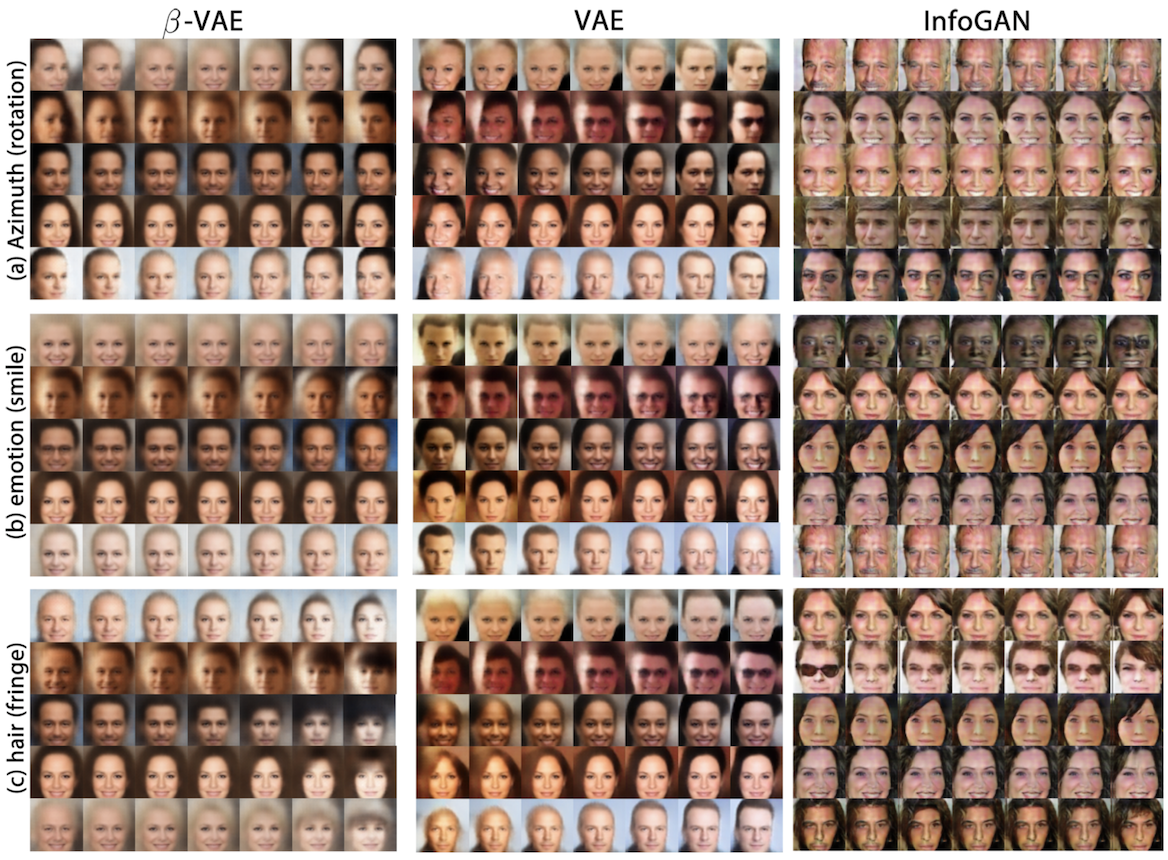
\includegraphics[width=0.95\linewidth]{figs/betaVAE_1.png}
\end{figure}
\vfill
\hrule\medskip
{\scriptsize \href{https://openreview.net/references/pdf?id=Sy2fzU9gl}{https://openreview.net/references/pdf?id=Sy2fzU9gl}}
\end{frame}
%=======
\begin{frame}{$\beta$-VAE, 2017}
\vspace{1cm}
\begin{figure}
    \centering
    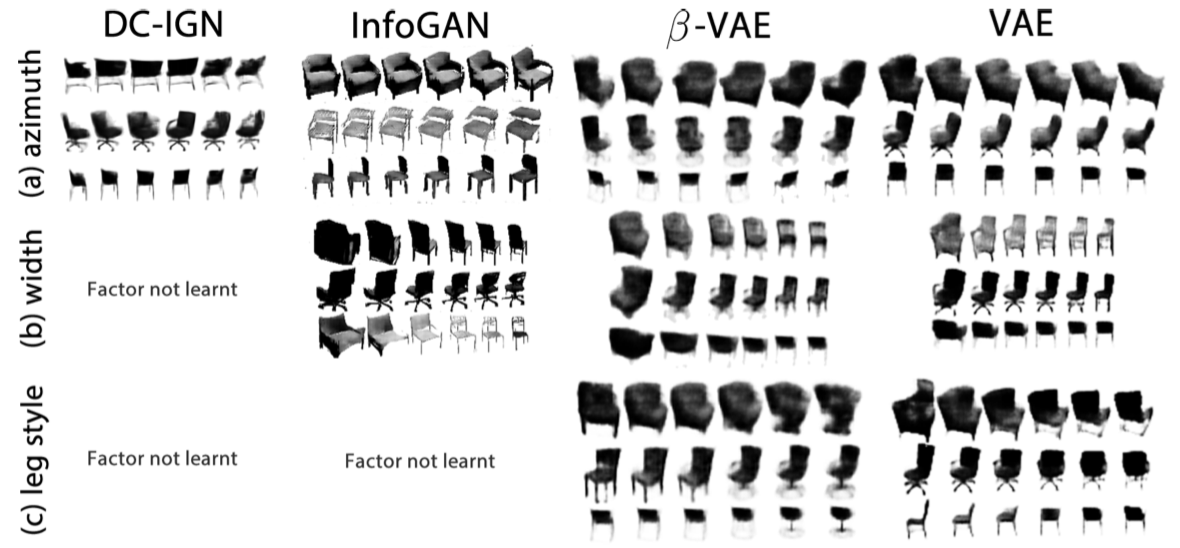
\includegraphics[width=\linewidth]{figs/betaVAE_2.png}
\end{figure}
\vspace{1cm}
\vfill
\hrule\medskip
{\scriptsize \href{https://openreview.net/references/pdf?id=Sy2fzU9gl}{https://openreview.net/references/pdf?id=Sy2fzU9gl}}
\end{frame}
%=======
\begin{frame}{$\beta$-VAE, 2017}
\begin{figure}
    \centering
    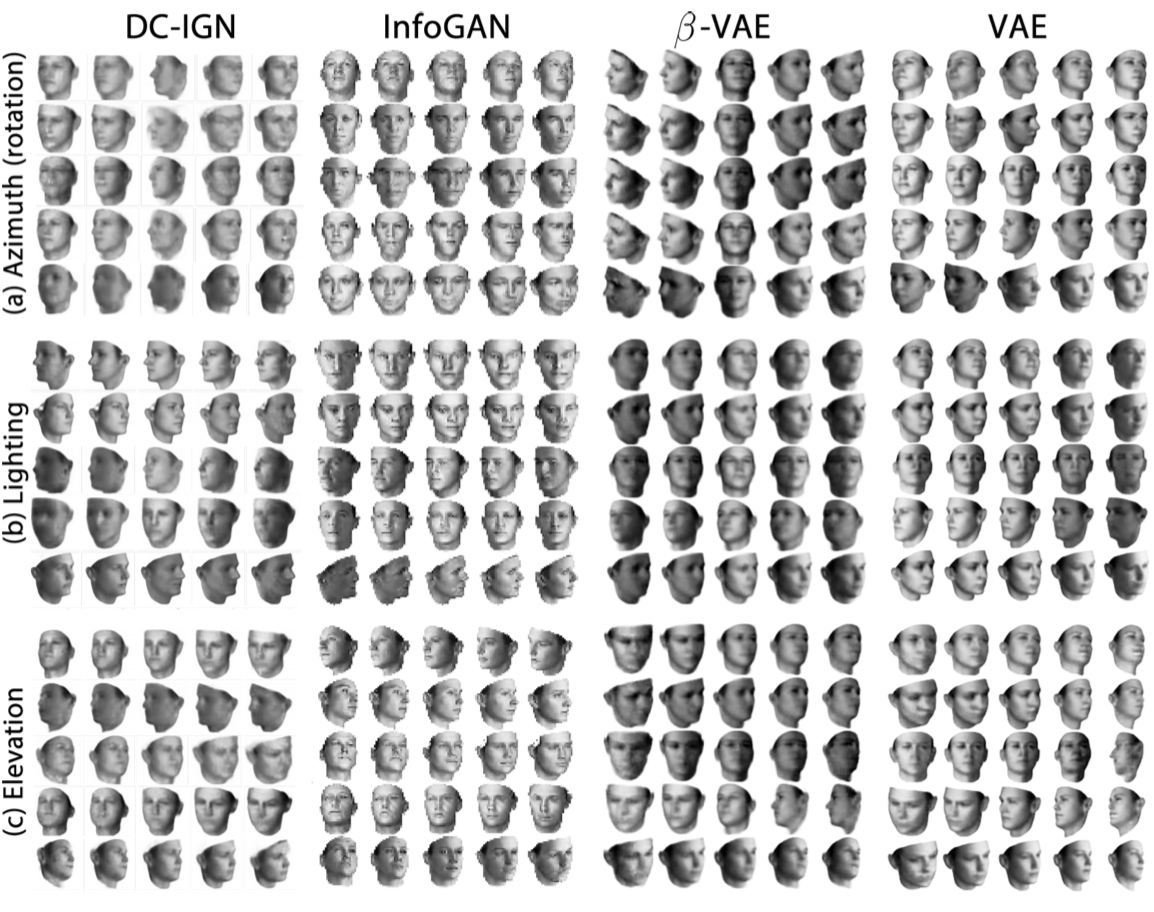
\includegraphics[width=0.8\linewidth]{figs/betaVAE_3.png}
\end{figure}
\vfill
\hrule\medskip
{\scriptsize \href{https://openreview.net/references/pdf?id=Sy2fzU9gl}{https://openreview.net/references/pdf?id=Sy2fzU9gl}}
\end{frame}
%=======
\begin{frame}{$\beta$-VAE, 2017}
	\begin{minipage}[t]{0.5\columnwidth}
	    \vspace{1.5cm}
		\begin{figure}
			\centering
			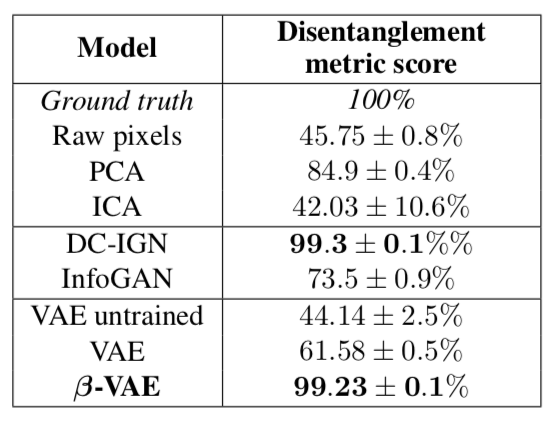
\includegraphics[width=1.\linewidth]{figs/betaVAE_4.png}
		\end{figure}
	\end{minipage}%
	\begin{minipage}[t]{0.5\columnwidth}
		\begin{figure}[h]
			\centering
			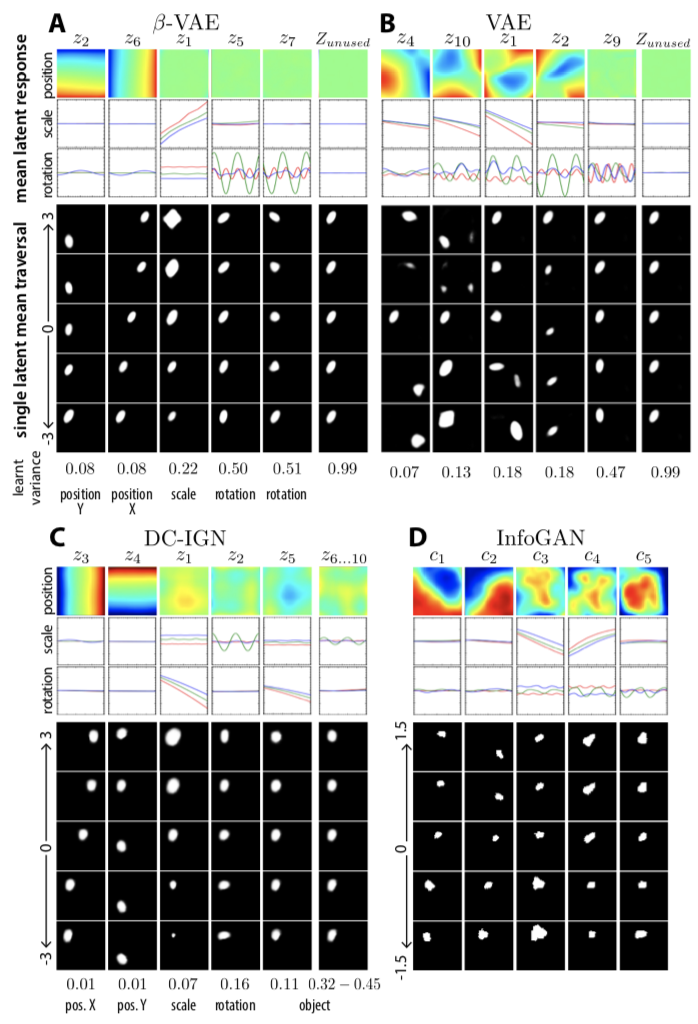
\includegraphics[width=.95\linewidth]{figs/betaVAE_5.png}
		\end{figure}
	\end{minipage}
\vfill
\hrule\medskip
{\scriptsize \href{https://openreview.net/references/pdf?id=Sy2fzU9gl}{https://openreview.net/references/pdf?id=Sy2fzU9gl}}
\end{frame}
%=======
\begin{frame}{$\beta$-VAE, 2018}
\begin{figure}
    \centering
    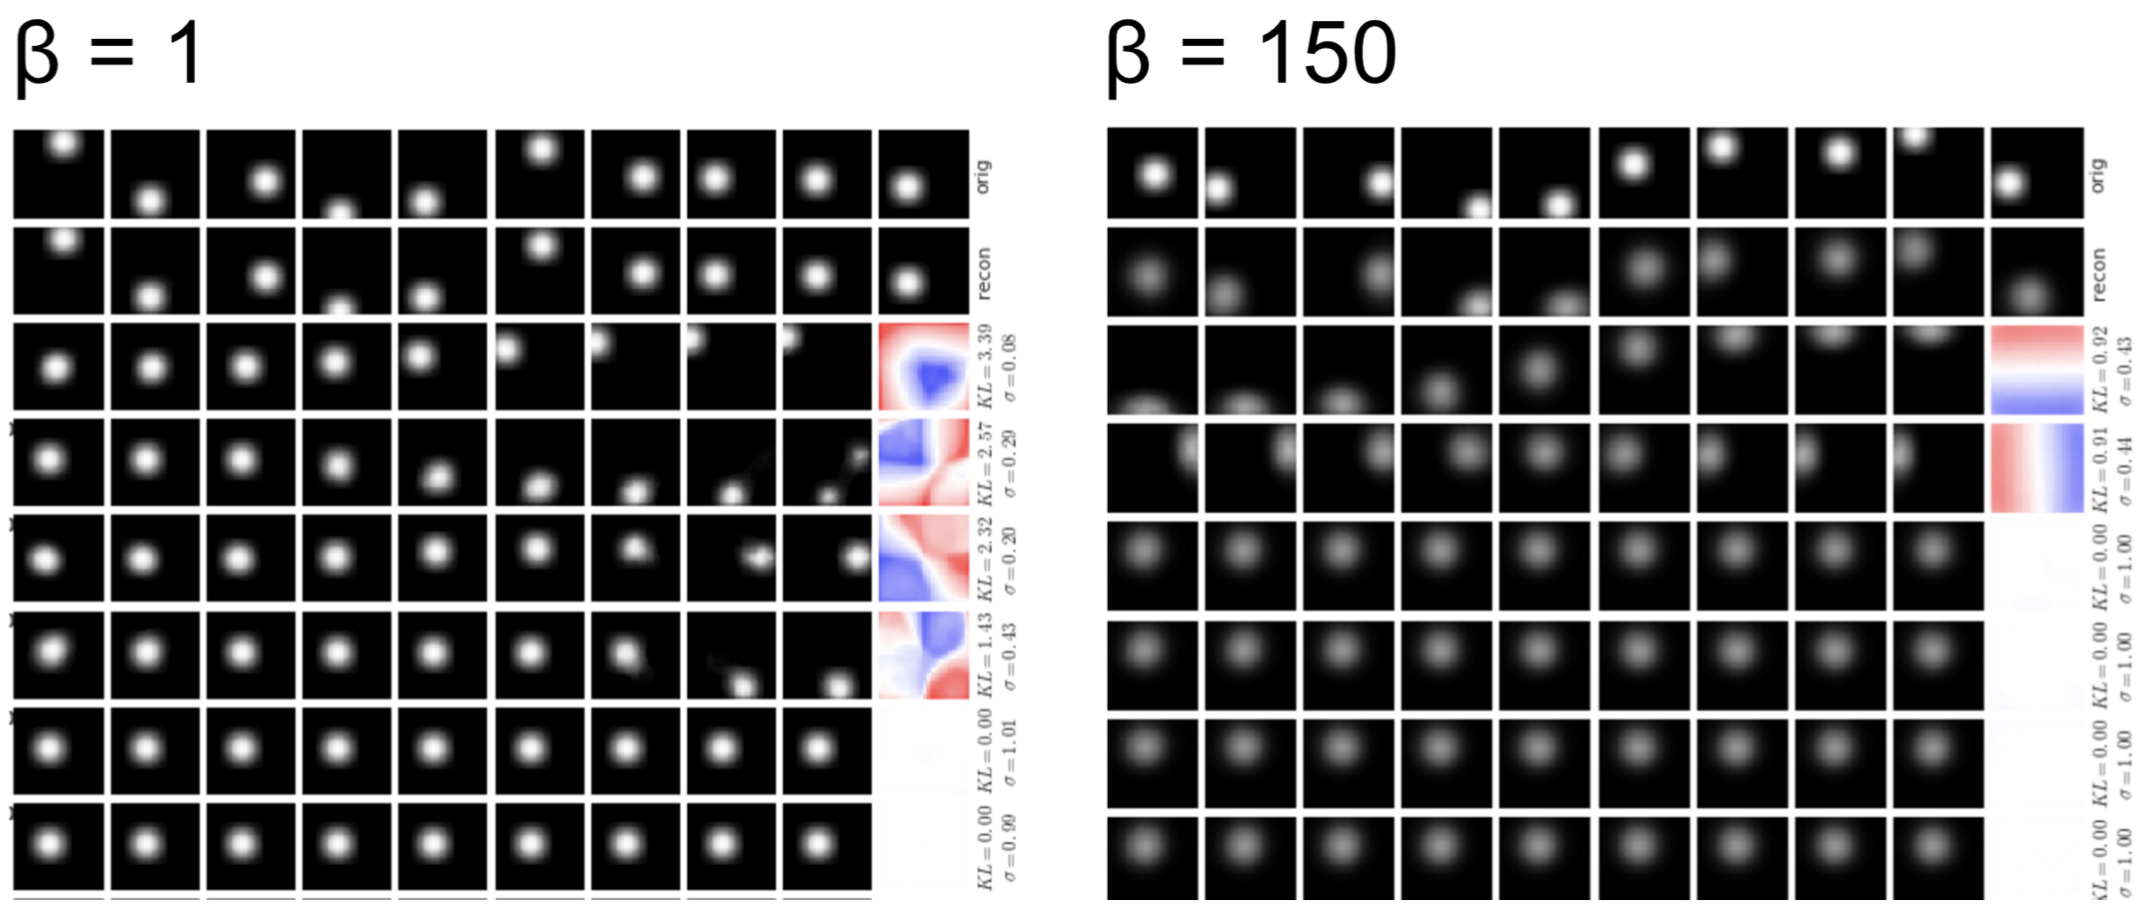
\includegraphics[width=\linewidth]{figs/betaVAE_6.png}
\end{figure}
\vfill
\hrule\medskip
{\scriptsize \href{https://arxiv.org/pdf/1804.03599.pdf}{https://arxiv.org/pdf/1804.03599.pdf}}
\end{frame}
%=======
\begin{frame}{$\beta$-VAE, 2018}
\begin{block}{Controlled encoding capacity}
\vspace{-0.5cm}
\[
    \mathcal{L}(q, \btheta, \beta) = \mathbb{E}_{q(\bz | \bx)} \log p(\bx | \bz, \btheta) - | KL (q(\bz | \bx) || p(\bz)) - C|.
\]
\end{block}
\begin{figure}
    \centering
    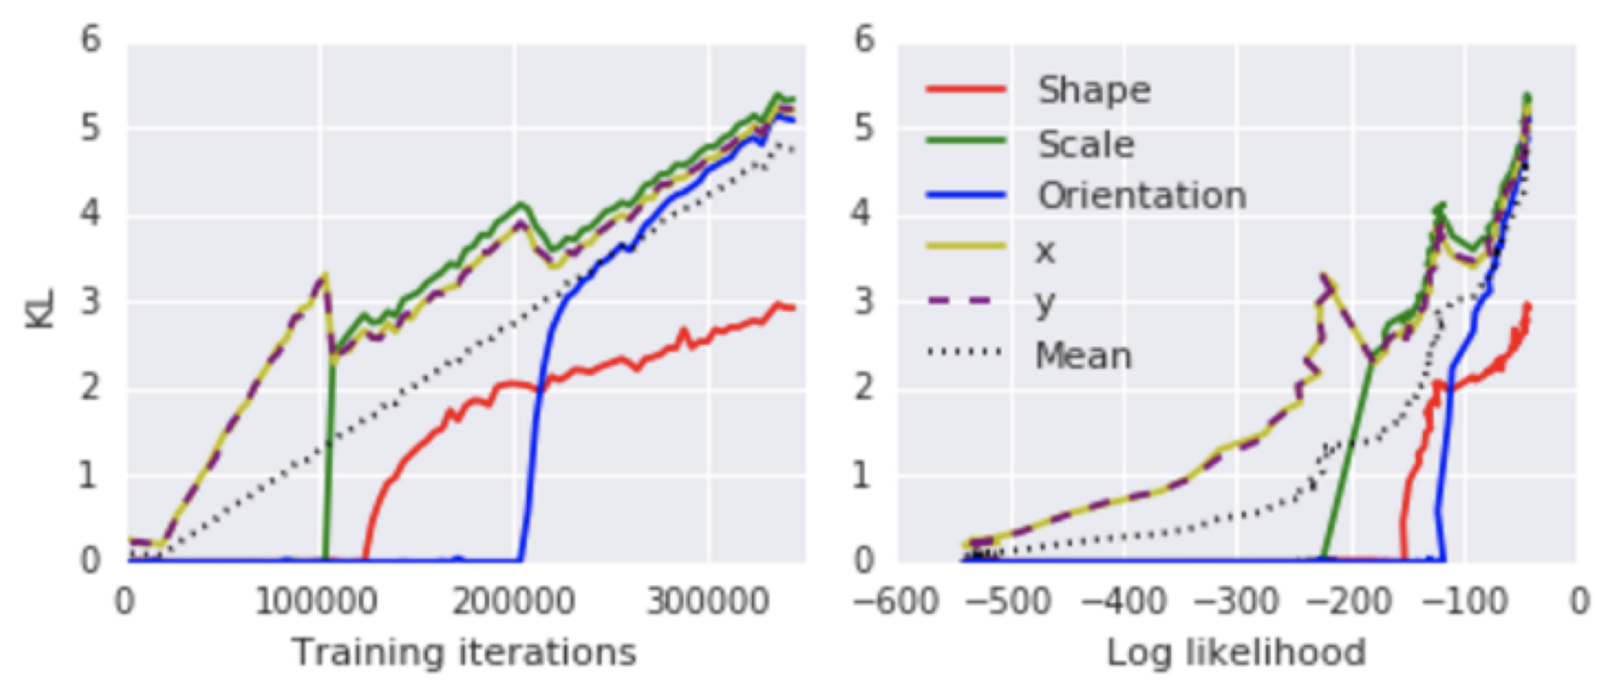
\includegraphics[width=\linewidth]{figs/betaVAE_7.png}
\end{figure}
\vfill
\hrule\medskip
{\scriptsize \href{https://arxiv.org/pdf/1804.03599.pdf}{https://arxiv.org/pdf/1804.03599.pdf}}
\end{frame}
%=======
\begin{frame}{$\beta$-VAE, 2018}
\begin{block}{Controlled encoding capacity}
\vspace{-0.5cm}
\[
    \mathcal{L}(q, \btheta, \beta) = \mathbb{E}_{q(\bz | \bx)} \log p(\bx | \bz, \btheta) - | KL (q(\bz | \bx) || p(\bz)) - C|.
\]
\end{block}
\begin{figure}
    \centering
    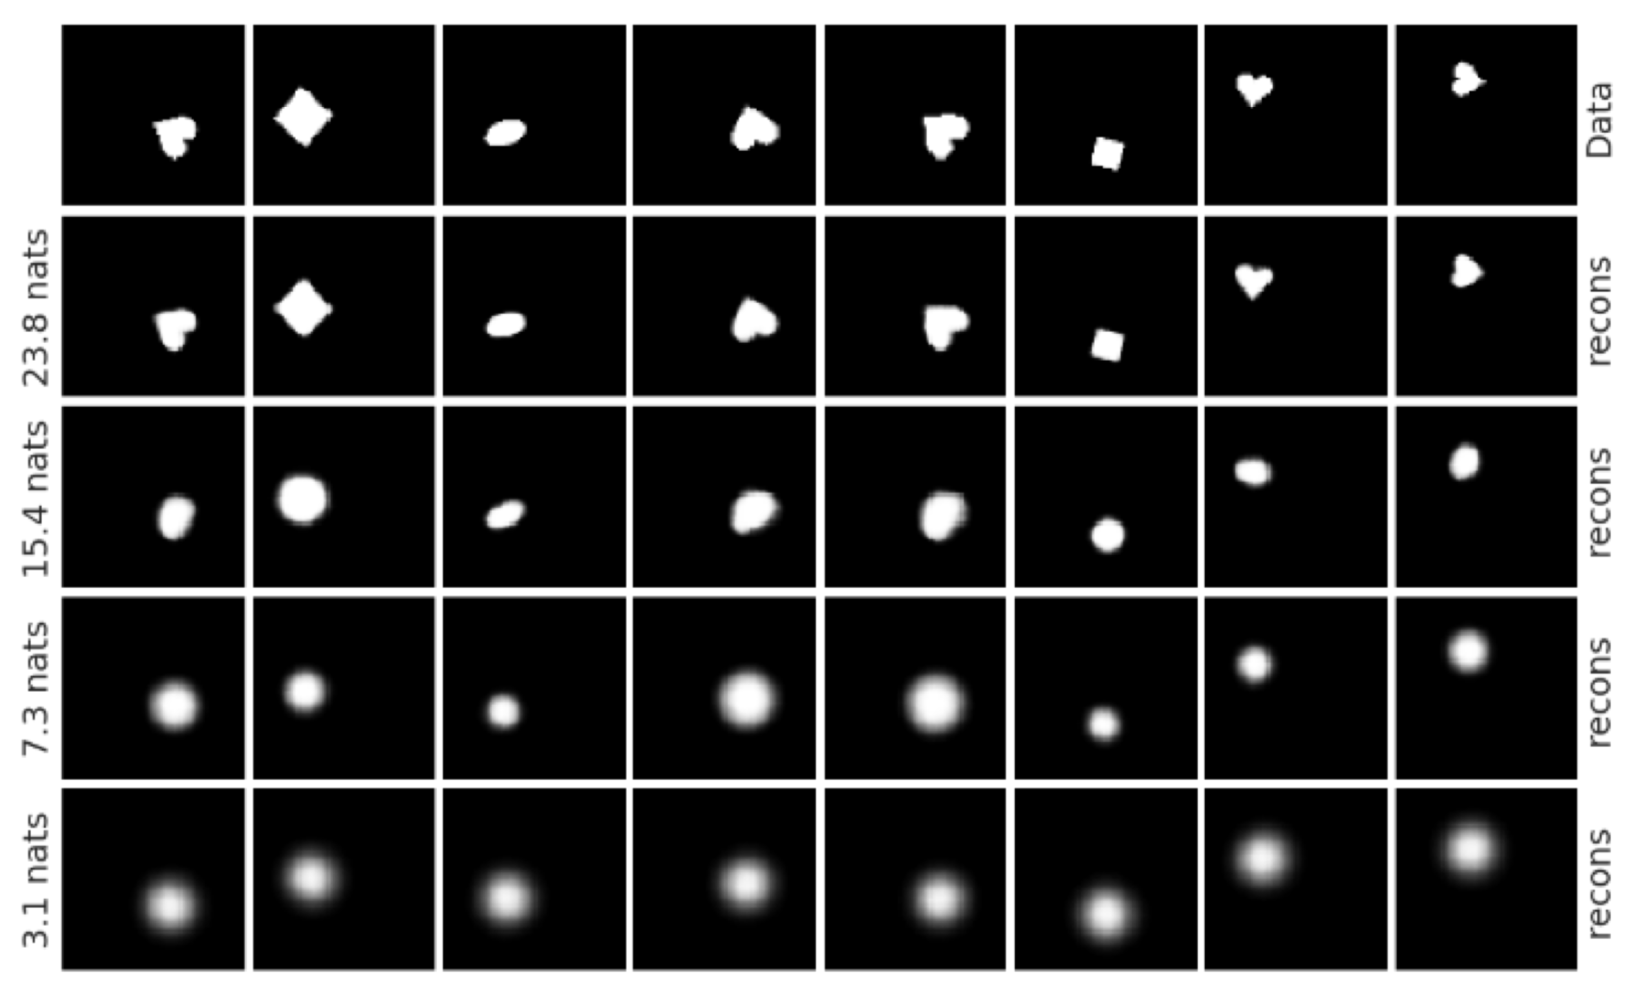
\includegraphics[width=0.8\linewidth]{figs/betaVAE_8.png}
\end{figure}
\vfill
\hrule\medskip
{\scriptsize \href{https://arxiv.org/pdf/1804.03599.pdf}{https://arxiv.org/pdf/1804.03599.pdf}}
\end{frame}
%=======
\begin{frame}{$\beta$-VAE, 2018}
\begin{figure}
    \centering
    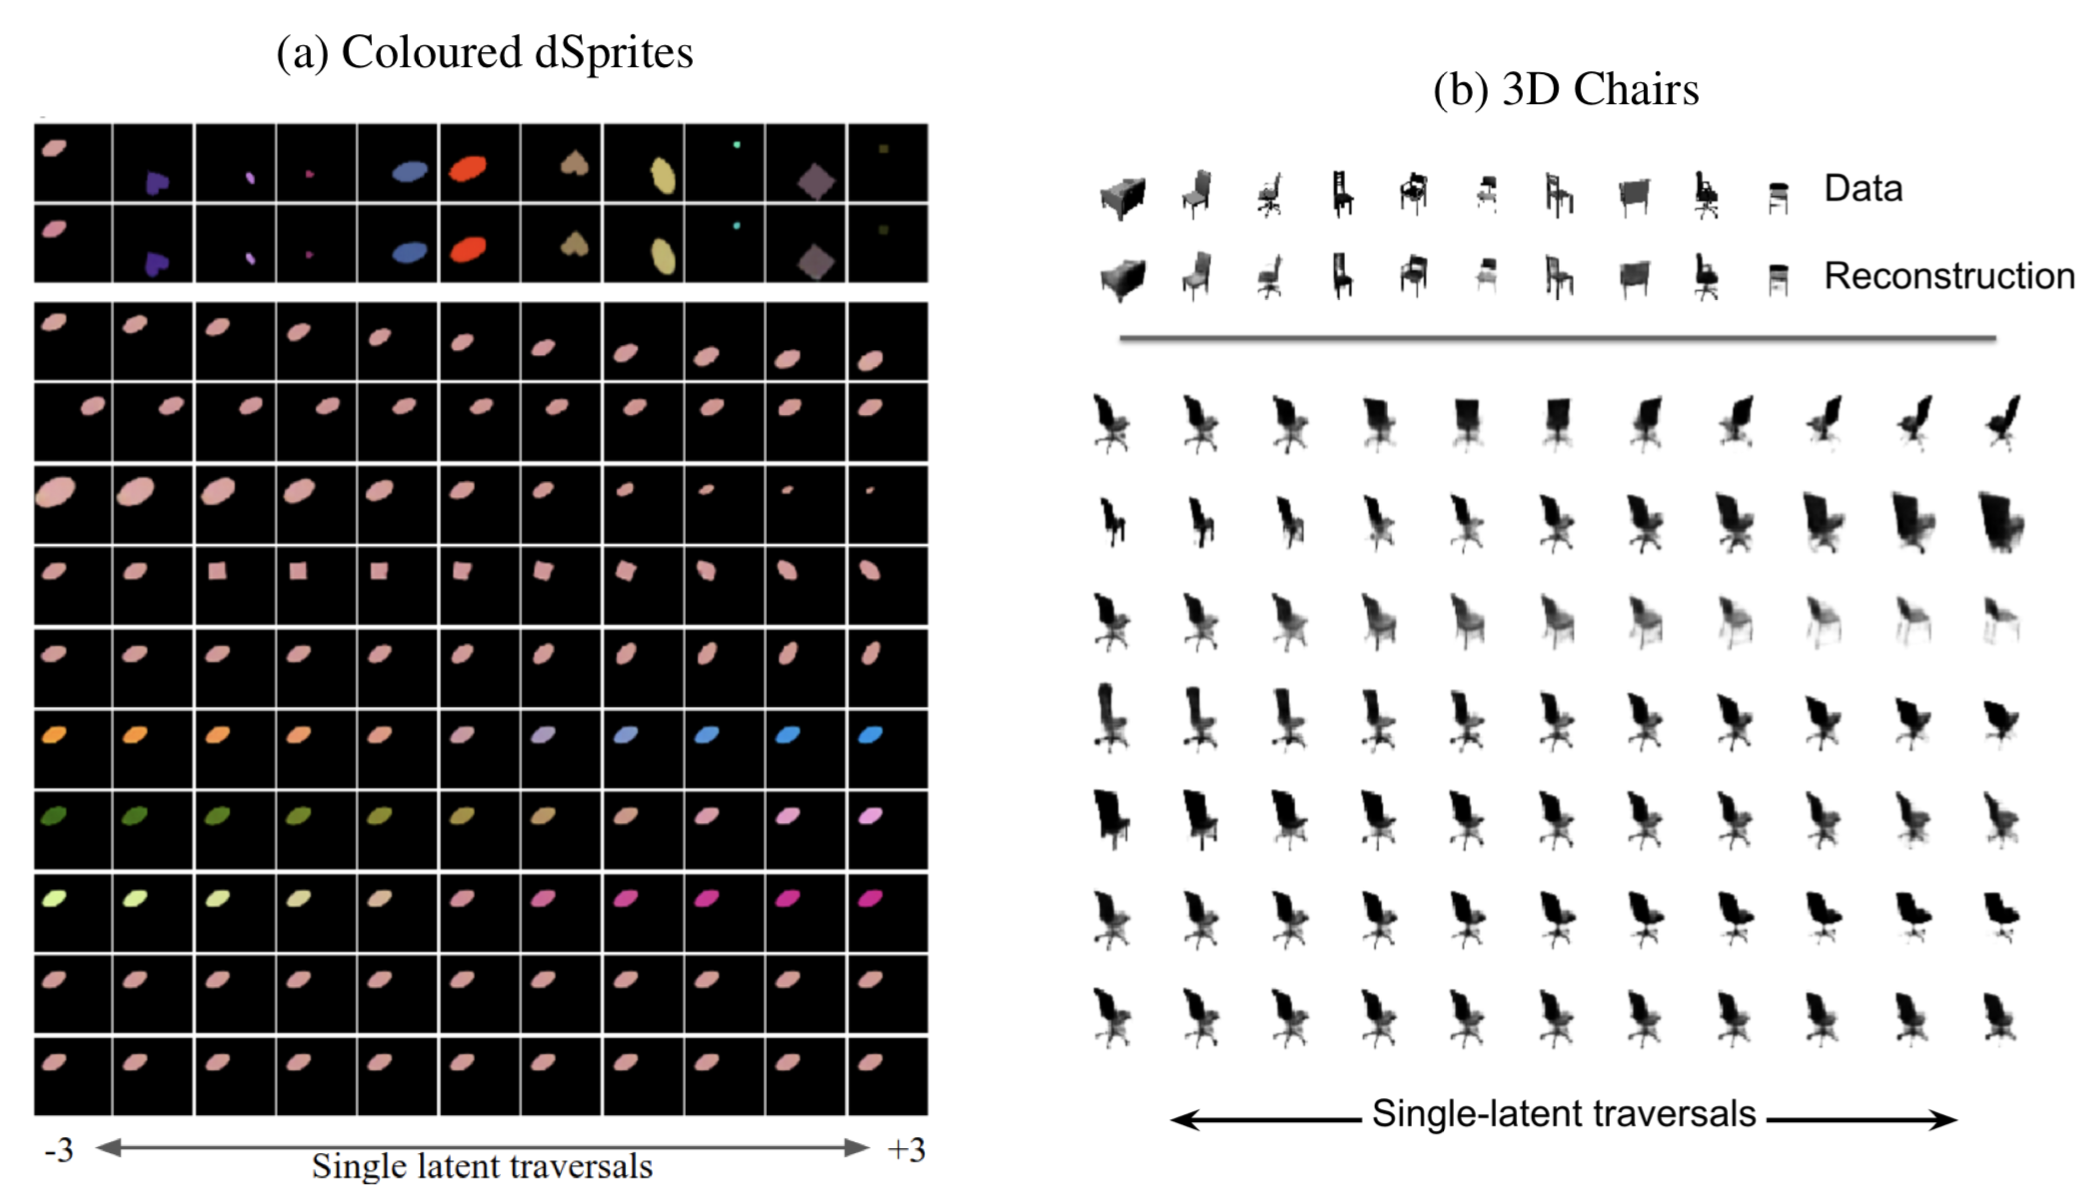
\includegraphics[width=\linewidth]{figs/betaVAE_9.png}
\end{figure}
\vfill
\hrule\medskip
{\scriptsize \href{https://arxiv.org/pdf/1804.03599.pdf}{https://arxiv.org/pdf/1804.03599.pdf}}
\end{frame}
%=======
\begin{frame}{DIP-VAE}
	
	\vfill
	\hrule\medskip
	{\scriptsize \href{https://arxiv.org/abs/1711.00848}{https://arxiv.org/abs/1711.00848}}
\end{frame}
%=======
\begin{frame}{FactorVAE}

	\vfill
	\hrule\medskip
	{\scriptsize \href{https://arxiv.org/abs/1802.05983}{https://arxiv.org/abs/1802.05983}}
\end{frame}
%=======
\begin{frame}{References}
{\tiny
\begin{itemize}
	
	\item \textbf{InfoGAN:} Interpretable Representation Learning by Information Maximizing Generative Adversarial Nets \\
	\href{https://arxiv.org/abs/1606.03657}{https://arxiv.org/abs/1606.03657} \\
	\textbf{Summary:} An information-theoretic extension to the GANs that disentangles representations in an unsupervised manner. InfoGAN maximizes the MI between a small subset of the latent variables and the observation. Lower bound for \\ MI objective is derived that can be optimized efficiently. 
    
    \item \textbf{beta-VAE:} Learning Basic Visual Concepts with a Constrained Variational Framework \\
    \href{https://openreview.net/references/pdf?id=Sy2fzU9gl}{https://openreview.net/references/pdf?id=Sy2fzU9gl} \\
    \textbf{Summary:} Modifications of VAE objective. The task is represented as constrained optimization. Increasing the \\ weight of KL divergence term in ELBO allows to disentangle latent space factors and makes model more interpretable. \\ The assessment of disentanglement is provided by constructing the classifier.
    
    \item Understanding disentangling in \textbf{$\beta$-VAE} \\
    \href{https://arxiv.org/pdf/1804.03599.pdf}{https://arxiv.org/pdf/1804.03599.pdf} \\
    \textbf{Summary:} Consider beta-VAE from the position of the rate-distortion theory (information bottleneck). Propose \\ the modified ELBO with controlled latent capacity.
    
    \item \textbf{DIP-VAE:} Variational Inference of Disentangled Latent Concepts from Unlabeled Observations \\
    \href{https://arxiv.org/abs/1711.00848}{https://arxiv.org/abs/1711.00848} \\
    \textbf{Summary:} Introduce a regularizer on the expectation of the approximate posterior over observed data that encourages \\ the disentanglement. Penalize the mismatch between the aggregated posterior and a factorized prior. Comparison with beta-VAE.
    
    \item \textbf{FactorVAE:} Disentangling by Factorising \\
    \href{https://arxiv.org/abs/1802.05983}{https://arxiv.org/abs/1802.05983} \\
    \textbf{Summary:} Penalizes the total correlation with density-ratio estimation. Comparison with beta-VAE. Does not degrate \\ the reconstructions.
\end{itemize}
}
\end{frame}
\end{document} 